% This must be in the first 5 lines to tell arXiv to use pdfLaTeX, which is strongly recommended.
\pdfoutput=1
% In particular, the hyperref package requires pdfLaTeX in order to break URLs across lines.

\documentclass[11pt]{article}

% package for adding images
\usepackage{graphicx}

%citation package
\usepackage{natbib}

% Remove the "review" option to generate the final version.
\usepackage{acl}

% Standard package includes
\usepackage{times}
\usepackage{latexsym}

% For proper rendering and hyphenation of words containing Latin characters (including in bib files)
\usepackage[T1]{fontenc}
% For Vietnamese characters
% \usepackage[T5]{fontenc}
% See https://www.latex-project.org/help/documentation/encguide.pdf for other character sets

% This assumes your files are encoded as UTF8
\usepackage[utf8]{inputenc}

% This is not strictly necessary, and may be commented out,
% but it will improve the layout of the manuscript,
% and will typically save some space.
\usepackage{microtype}

% If the title and author information does not fit in the area allocated, uncomment the following
%
%\setlength\titlebox{<dim>}
%
% and set <dim> to something 5cm or larger.

\title{English and Arabic Sarcasm Detection in Tweets}

% Author information can be set in various styles:
% For several authors from the same institution:
% \author{Author 1 \and ... \and Author n \\
%         Address line \\ ... \\ Address line}
% if the names do not fit well on one line use
%         Author 1 \\ {\bf Author 2} \\ ... \\ {\bf Author n} \\
% For authors from different institutions:
% \author{Author 1 \\ Address line \\  ... \\ Address line
%         \And  ... \And
%         Author n \\ Address line \\ ... \\ Address line}
% To start a seperate ``row'' of authors use \AND, as in
% \author{Author 1 \\ Address line \\  ... \\ Address line
%         \AND
%         Author 2 \\ Address line \\ ... \\ Address line \And
%         Author 3 \\ Address line \\ ... \\ Address line}

\author{Amy Tzu-Yu Chen \\
  University of Washington \\
  \texttt{amy17519@uw.edu} \\\And
  {David Roesler \\
  University of Washington \\
  \texttt{droesl@uw.edu} \\} \\\AND
  {Diana Baumgartner-Zhang \\
  University of Washington \\
  \texttt{diazhang@uw.edu} \\} \\\And
  Juliana McCausland \\
  University of Washington \\
  \texttt{jumc1469@uw.edu} \\}

\begin{document}
\maketitle
\begin{abstract}


Sarcasm detection is a task that has grown in importance over the last few years due to the negative impact that sarcasm has on sentiment classification systems \citealp{Liu2010SentimentAA}. Sarcasm is inherently difficult to identify because of its form. Here we propose a method to classify sarcasm in tweet text as part of the iSarcasmEval 2022 task. For our approach, we use a BERTweet encoder. Our primary model outperforms the top scoring submissions to the iSarcasmEval task 6A.
\end{abstract}

\section{Introduction}

In any text format, detecting whether someone is sarcastic or serious can be challenging. For spoken interactions, we can rely on intonation, facial expressions, and other non-verbal cues to inform us on the underlying meanings. On Twitter or other social media platforms, users often express their opinions or thoughts solely through text. Discerning whether a text should be interpreted literally or figuratively can prove to be a challenge for humans, and even more so for a machine.

The use of sarcasm on the internet is ubiquitous, and its presence can disrupt computational systems of sentiment analysis, which are widely used in industry \citealp{Liu2010SentimentAA}. As a result, it has become essential to build systems that can detect sarcasm. Previous work in this area relies on distant supervision methods that use features like hashtags to indicate whether or not a text is sarcastic. This can lead to noisy data that inevitably produces false positives. Other commonly used approaches rely on the manual labeling of text data. This often requires third-party annotators and can result in problems of annotator agreement.

\section{Task Description}

Our primary task is sarcasm detection in English Twitter text, which we treat as a binary classification problem. Given a text, our task is to determine whether it is sarcastic or non-sarcastic. Sarcasm is a form of verbal irony through which a speaker expresses their stance toward a topic, which often takes the form of contempt or derogation \citealp{WILSON20061722}. Automatic sarcasm detection \citealp{joshi:automatic} is the prediction of the presence of sarcasm in text. 

Twitter, a platform often used to express the critical viewpoints of its users, has been a common data source for sarcasm detection models \citealp{doi:10.1177/1470785320921779}. To train and evaluate our model, we make use of the Twitter sarcasm dataset from SemEval 2022 Task 6, iSarcasmEval \citealp{oprea-magdy-2020-isarcasm}. 

Unlike sarcasm datasets labeled by third-party annotators, the iSarcasm dataset contains labels provided by the authors of the tweets themselves. The iSarcasm dataset thus represents instances of intended sarcasm, in which the sarcastic intention of the author may not align with the perceptions of their readers. As demonstrated in \citealp{oprea-magdy-2020-isarcasm}, instances of intended sarcasm can be more difficult to detect than instances of perceived sarcasm. 

The iSarcasmEval shared task data includes both English and Arabic sets. As our secondary adaptation task, we perform sentiment detection on the Arabic portion of the dataset. To evaluate the performance of our binary classification model, we measure F1 score on the positive (sarcastic) class.

\section{System Overview}
\subsection{Initial System}

In our initial sarcasm detection model, we fine-tune BERTweet \citealp{nguyen-etal-2020-bertweet} on the iSarcasmEval training data. As illustrated in \ref{fig:overview-class-model}, we attach a classifier head (a pair of fully-connected layers with a softmax output) to the BERTweet base model. The classifier head produces a sarcasm prediction for each input tweet using the [CLS] token representation produced by the BERTweet encoder. 

\begin{figure}[h!]
    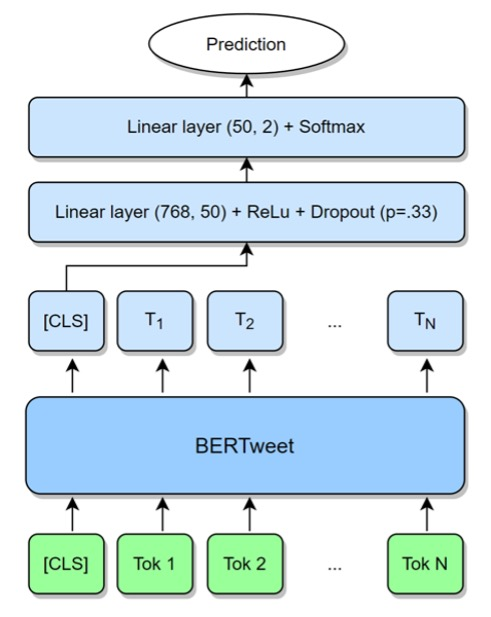
\includegraphics[width=.5\textwidth]{Picture1.jpg}
    \caption{Overview of classification model}
    \label{fig:overview-class-model}
\end{figure}

\subsection{Revised System}

In our revised sarcasm detection system, we change the encoder component of our system from a BERTweet-base to a BERTweet-large model. The BERTweet-large model has the same structure as RoBERTa-large \citealp{devlin2018bert}, which produces 1024-dimensional output representations, rather than the 768-dimensional outputs produced by the base version of the model. We modify our classifier head to match the output size of BERT-large and also increase the size of the hidden layer from 50 to 100 neurons. 

To create our system’s sarcasm predictions, we create an ensemble of five BERTweet-large models, depicted in \ref{fig:overview-ensemble-model}. Each of the models in the ensemble are fine-tuned on our original training set, augmented with a different random sampling of tweets from the English sarcastic tweet dataset produced by \citealp{Ptcek2014SarcasmDO}. Our ensembling strategy is variance reduction through bootstrap aggregation, or bagging, where hard majority voting is used to create the final system predictions.

\begin{figure}[h!]
    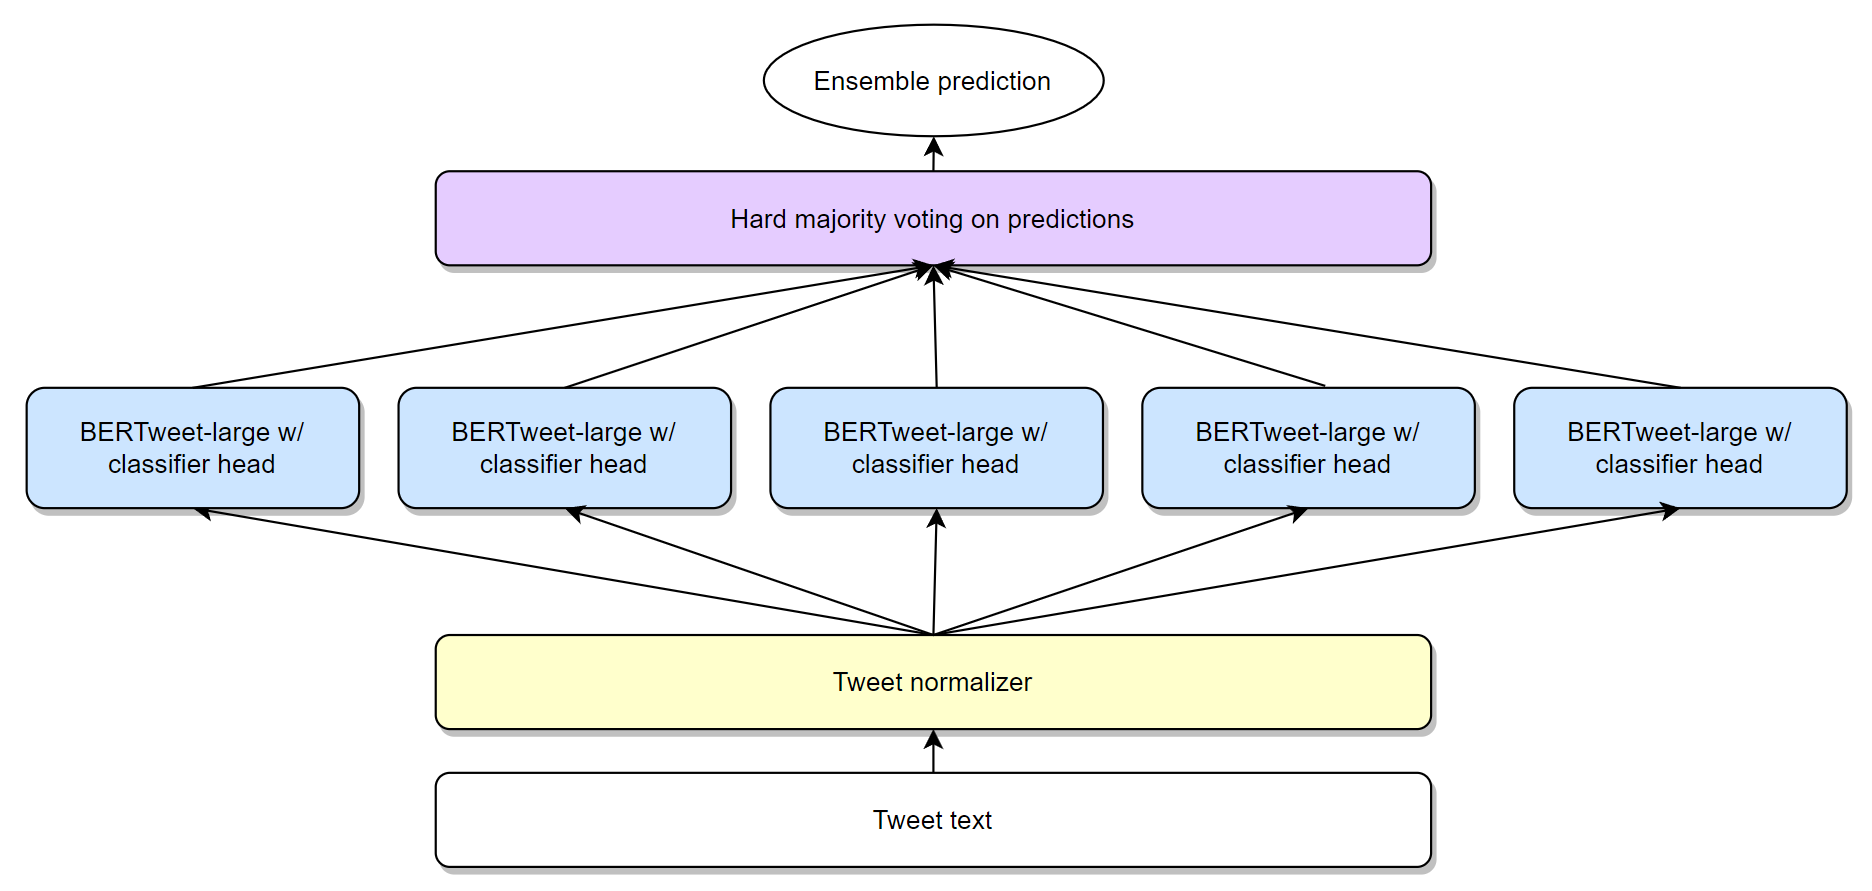
\includegraphics[width=.5\textwidth]{Picture8.png}
    \caption{Overview of ensemble model}
    \label{fig:overview-ensemble-model}
\end{figure}

\subsection{Adaptation System}
For our adaptation system, we fine-tune CamelBERT-mix \citealp{inoue2021interplay} on iSarcasmEval’s Arabic training data. We attempted to keep the architecture similar to the initial English system, with a classifier head and hidden layer of size 50, but also added two additional linear layers with dimensions of 25 and 10. The classifier head produces a sarcasm prediction for every input.


\section{Approach}
\subsection{Initial Approach}
The tweets included in iSarcasmEval dataset exhibit typical characteristics of Twitter text, which is short in length (due to character limits) and contains frequent use of informal grammar and irregular vocabulary, such as abbreviations and hashtags. Additionally, the iSarcasmEval data is rich in emoticons and emoji, both of which are used by social media users as nonverbal cues to indicate sarcastic intent \citealp{doi:10.1080/17470218.2015.1106566}.

In order to leverage the unique grammatical, lexical, and symbolic characteristics of tweets in our classification system, we utilize BERTweet, a large-scale language model trained on 850M tweets, as our encoder. To preserve emoji information in inputs, we first normalize tweets using the tweet normalizer function used in the BERTweet pre-training by Nguyen et al. The tweet normalizer (\ref{fig:example-tweet-normalization}) converts emoji into text strings, user mentions into '@USER', and web links into 'HTTPURL'.

\begin{figure}[h!]
    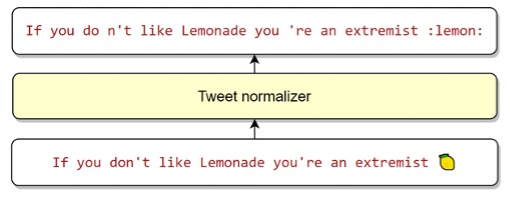
\includegraphics[width=.5\textwidth]{Picture2.jpg}
    \caption{Example tweet normalization}
    \label{fig:example-tweet-normalization}
\end{figure}

We balance the number of positive and negative examples of sarcasm in our dataset by including all examples of the positive class and randomly sampling an equal number from the negative class. For fine-tuning, we use a single Tesla P100 GPU on the Google Colab platform. Pytorch and the Huggingface library are used to fine-tune BERTweet on the iSarcasmEval training set for five training epochs. We use AdamW(\citealp{https://doi.org/10.48550/arxiv.1711.05101}) with a learning rate of 5.e-5 (controlled by a learning rate scheduler) and a batch size of 32.

As our baseline models, we use Random Forest and LightGBM \citealp{ke2017lightgbm} to perform binary classification for predicting sarcasm. In the preprocessing step, we use the sci-kit learn package \citealp{DBLP:journals/corr/abs-1201-0490} TfidfVectorizer with ngram range set to (2, 6) which considers bigrams to six-grams. After vectorization, we run Random Forest and LightGBM using the same balanced training data set.


\subsection{D3 Revised Approach}
\subsubsection{D3 Submitted System}
In our revised approach we create sarcasm predictions for each tweet using an ensemble of BERTweet-large classifiers. Each of the five classifiers is trained on our original balanced training set created from the iSarcasmEval training data \citealp{oprea-magdy-2020-isarcasm}. Additionally, the training set for each of the classifiers is augmented with a random sampling of 800 positive and 800 negative tweets from the Twitter sarcasm dataset produced by \citealp{Ptcek2014SarcasmDO}. 

The  \citealp{Ptcek2014SarcasmDO} data differs from the iSarcasmEval data in that sarcastic tweets were identified through distant supervision (hashtags such as #sarcasm) rather than author identification. Additionally, the \citealp{Ptcek2014SarcasmDO} data is roughly six years older than the iSarcasm set and does not contain more recent lexical innovations, such as terms related to COVID-19 and covid vaccination.

We fine-tune each of the BERTweet-large sub-models on a single Tesla P100 GPU on the Google Colab platform using the AdamW optimizer with a learning rate of 3e-6 (controlled by learning rate scheduler) and a batch size of 32. We train for 30 epochs and retain the checkpoint where the model achieves the highest F1 score on the positive (sarcastic) class. When fine-tuning each of our ensemble sub-models, we also utilize thresholding \citealp{sheng-threshold} to identify the optimal threshold for best positive class F1. 

The logits output of each sub-model are passed through a softmax function and predictions for each sub-model are determined using the best probability threshold for that model. The predictions for each sub-model are aggregated and the final ensemble predictions are determined by hard voting. 

\subsubsection{D3 Experiments}
In our system revision process, we also experimented with several changes that were not included in our final submitted system.

We combined the BERTweet [CLS] output with fine-tuned DeepMoji \citealp{felbo-etal-2017-using} representations of the tweet and used the combined representations as the input to the classifier head. This method provided minimal improvements when combined with the BERTweet-base model and no improvement when combined with BERTweet-large, and was not included as a component of our final system.

To supplement our data, we also attempted the addition of the Self-Annotated Reddit Corpus (SARC) \citealp{khodak-etal-2018-large}. Ultimately, we did not use this dataset in our revised system. We felt the dataset was not suitable to the task and current system for the following reasons: 1) The length of a Reddit post can be much longer than a tweet and only those posts that were equal to or less than the length of a tweet could be used as BERTweet inputs; and 2) Emojis and hashtags are less frequent in Reddit data, which results in text features unlike those of our training and validation sets.

\subsection{D4 Approach}
\subsubsection{D4 Primary Task}
In the second round of revisions, we tested a variety of strategies for improving performance on the primary task. However, none of these methods resulted in improvements to our D3 model and thus were not included in our final system.

First, we added additional features derived from the tweets. We concatenated additional features to the BERTweet-large encoder outputs and then passed the concatenated vector to the classifier head. These additional features included sentiment scores for each tweet from the Vader package \citealp{Hutto2014VADERAP}, the TextBlob package, EAISe affect vectors \citealp{babanejad-etal-2020-affective}, and our own rule-based features (such as the absence or presence of multiple exclamation marks or multiple question marks in the tweets). The addition of these features in isolation or combination provided no improvement to our D3 model. We speculate that the majority of these affect-based or punctuation-based features may have already been encoded by the BERTweet-large model and thus did not provide the system with any additional leverage.

Second, we modified the ensembling method from D3. We changed our ensemble voting mechanic from hard voting on sub-model predictions to soft voting, where probabilities produced by each sub-model are averaged in order to determine the final prediction. This method did not perform as well on our validation set, most likely due to our use of threshold moving during sub-model training. We also created a stacking ensemble where a 'meta-learner' linear layer (trained on the validation set) learns a weighting system for the predictions of each sub-model. This method resulted in over-fitting on our validation data and did not generalize well to the test set.

Third, we replaced the model’s classifier head. We also experimented with replacing the MLP classifier head with one of our baseline classifiers, LightGBM \citealp{ke2017lightgbm}. We first fine-tuned BERTweet-large with the original MLP classifier head on our training data, then retrieved the encoded representations of our training data from the CLS token of the fine-tuned BERTweet model. These vectors and their class labels were then used to train a LightGBM classifier. This method performed relatively poorly in comparison with the original method of simultaneously fine-tuning the encoder and classifier head.

\subsubsection{D4 Adaptation Task}
For the adaptation model, we intended to keep the architecture similar to that of our primary task. However, modifying the English model to take in Arabic inputs would have been a challenge (i.e. do we translate Arabic text to English? How do we do the translation? Does this cause auto translate issues?). Instead, we attempted fine-tuning on two different BERT models trained specifically on Arabic text: CamelBERT-mix \citealp{inoue2021interplay} and MARBERT \citealp{DBLP:journals/corr/abs-2101-01785}.Our final submission for D4 uses CamelBERT-mix. 

We trained all versions on patas (gn3, Quadro 8000), the UW Linguistics shared computing resources. 


\section{Results}
\subsection{Initial Results}

\begin{figure}[h!]
    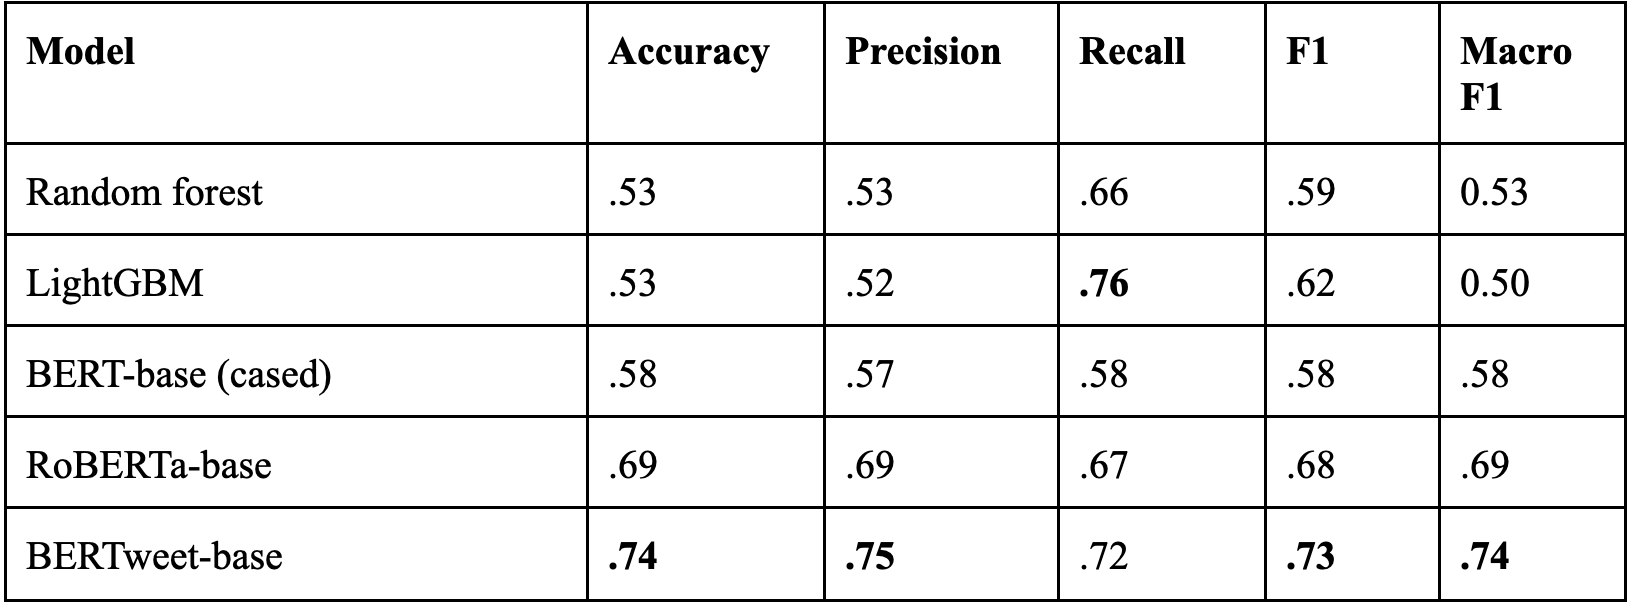
\includegraphics[width=.5\textwidth]{Picture3}
    \caption{Validation results for positive (sarcastic) class}
\end{figure}

When evaluating our baseline models on our validation set, we find that the Random forest and LightGBM models perform similarly, with Random forest reaching a positive class F1 score of .59, and LightGBM reaching .62 F1. We also evaluate a fine-tuned BERT-based (cased) on our validation set and find that this model achieves a lower F1 score than our baseline models, although it achieves a slightly higher Macro F1 score. When evaluating a fine-tuned RoBERTa-base model, we see a noticeable improvement across the board. 

When evaluating a fine-tuned BERTweet-base model, an encoder specifically pre-trained on tweet data, we find that of the models tested, this model performs best. The fine-tuned BERTweet-based achieves a .73 F1 score for the positive class, with improved accuracy, and precision scores compared to the other models. The fine-tuned BERTweet-base model did, however, achieve a lower recall score than the LightGBM baseline.

\subsection{D3 Revised Results}
\begin{figure}[h!]
    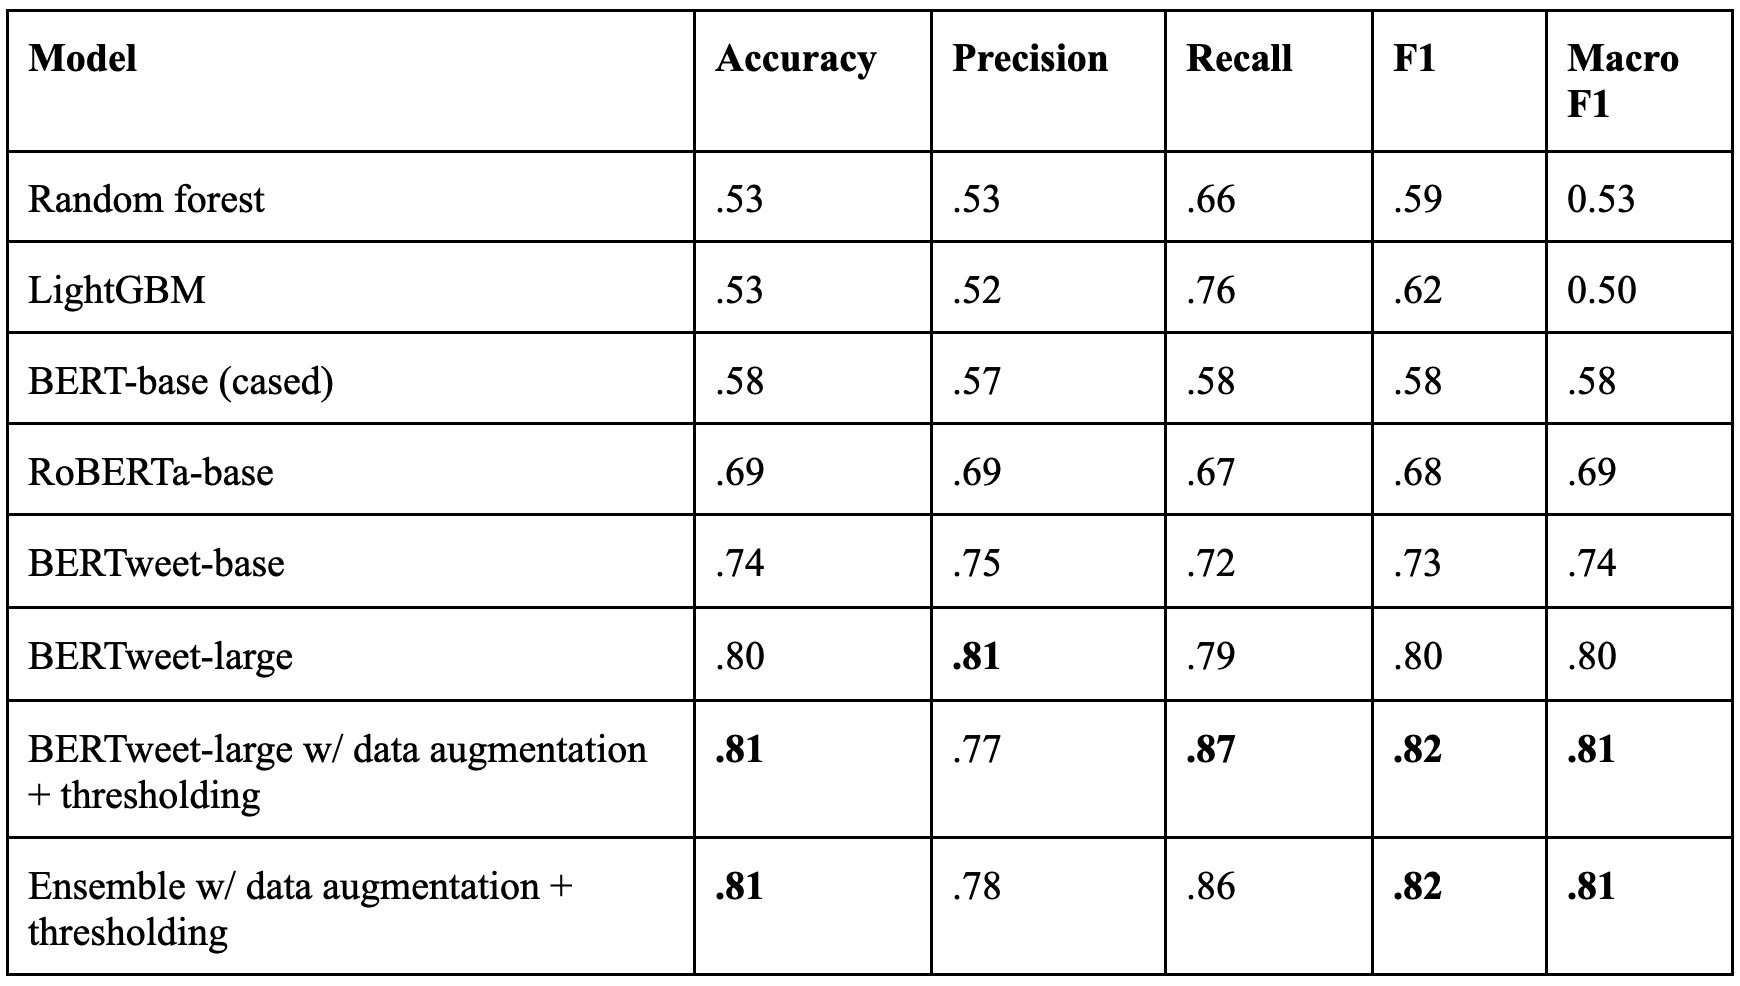
\includegraphics[width=.5\textwidth]{Picture9.png}
    \caption{Revised system validation results for positive (sarcastic) class}
\end{figure}

In our revised system, we fine-tune BERTweet-large on our training data, and when evaluating on our validation set, see an improved positive class F1 score of .80; an increase of .07 when compared to the fine-tuned BERTweet-base model. After incorporating data augmentation from \citealp{Ptcek2014SarcasmDO} dataset along with threshold moving to maximize positive class F1, the best single model of our BERTweet-large ensemble reaches 82 F1 for the positive class. The five-classifier BERTweet-large ensemble (with data augmentation and thresholding) also reaches 82 F1 for the positive class, which provides no improvement over the best single model in the ensemble. The lack of improvement from our ensembling strategy may be due to the very similar errors made by all of the sub-models, which included tweets that were either apparently sarcastic, but not labeled as such, or tweets which may have required additional world knowledge in order to identify as sarcasm. We further discuss these complications in our error analysis (Sec. 6.2). 

\subsection{D4 Revised Results}
\subsubsection{Primary Task Results}
\begin{figure}[h!]
    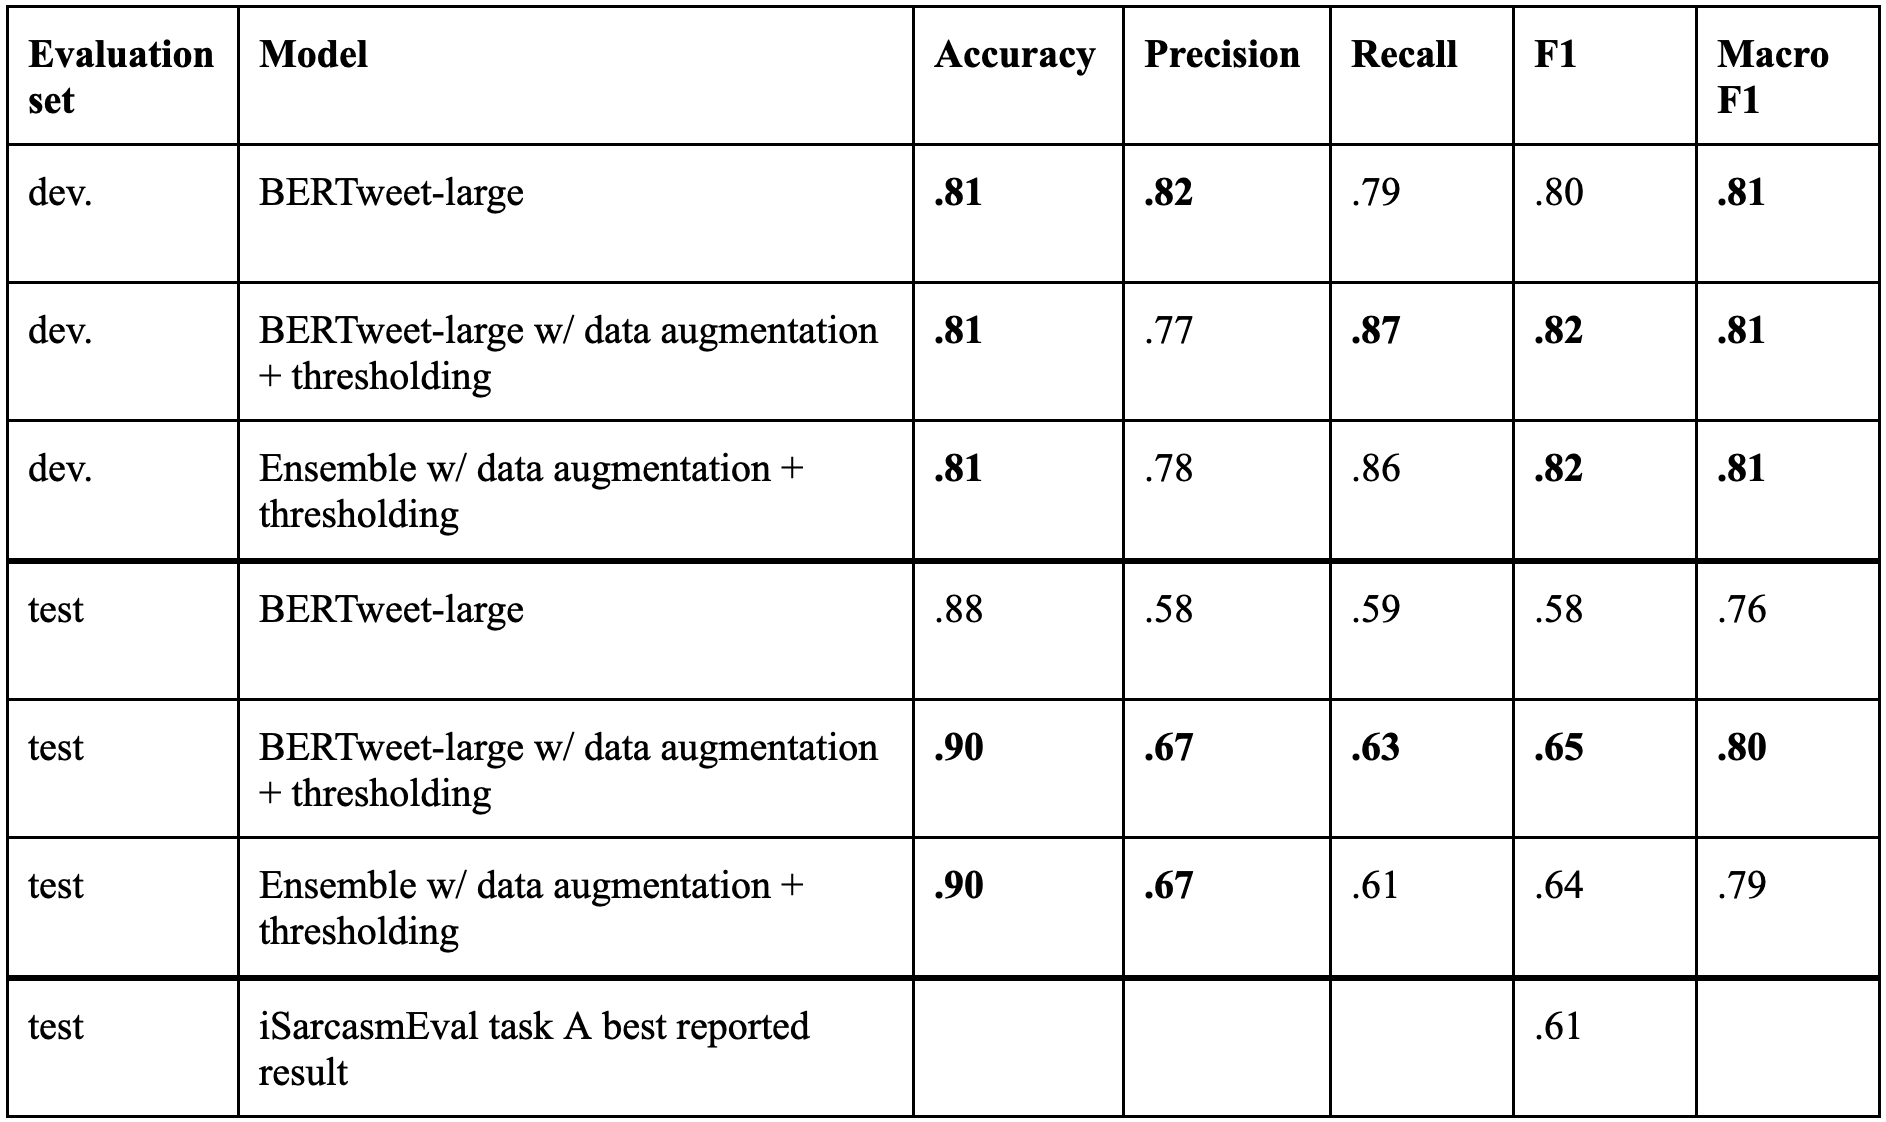
\includegraphics[width=.5\textwidth]{Primary system results for positive (sarcastic) class.png}
    \caption{Primary system results for positive (sarcastic) class}
\end{figure}

When evaluating a fine-tuned BERTweet-large model on the iSarcasm Task 6A English test set, we find that the model achieves .58 F1 for the positive class. The best single model of our ensemble, augmented with data from \citealp{Ptcek2014SarcasmDO} dataset and incorporating threshold moving, achieves an F1 score of .65, which outperforms the highest submitted score to the iSarcasm shared task by 4 F1 points. Our ensemble, with data augmentation and threshold moving, reaches .64 F1, slightly below the score of the best single model. When evaluating on the test data, we also find that our ensemble sub-models again make similar errors to one another, often on tweets that are intended as sarcastic, but may lack sufficient contextual clues for the models to leverage.  


\subsubsection{Adaptation Task Results}
\begin{figure}[h!]
    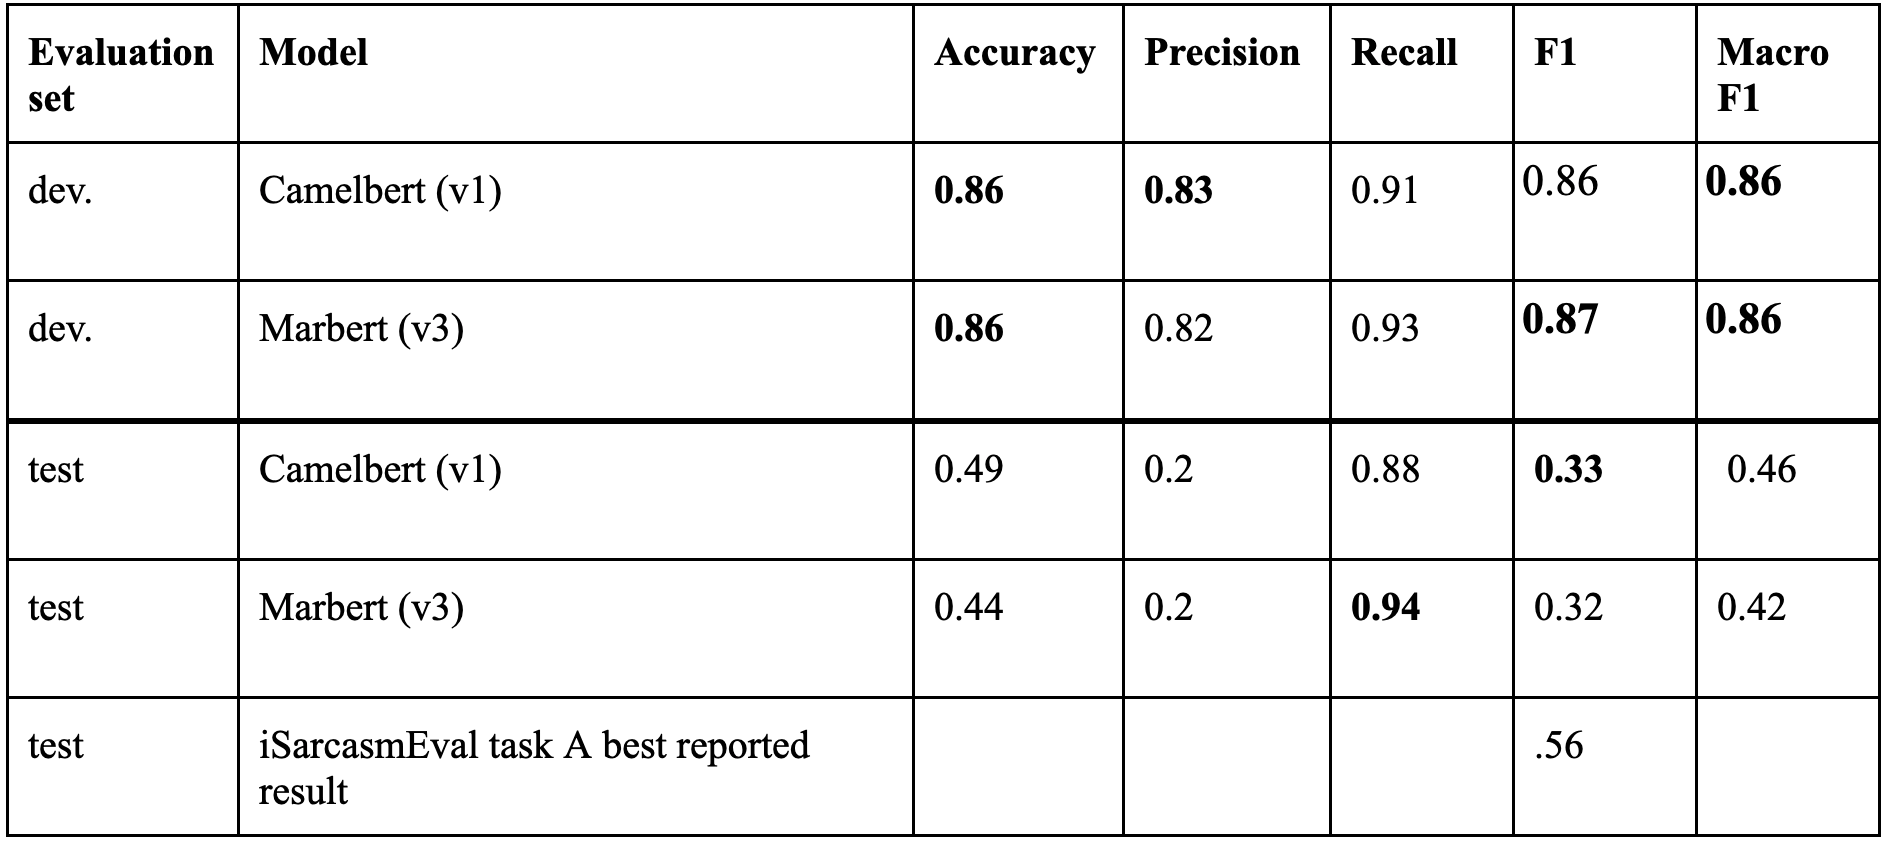
\includegraphics[width=.5\textwidth]{Adaptation system results for positive (sarcastic) class.png}
    \caption{Adaptation system results for positive (sarcastic) class}
\end{figure}

After adjusting the model for the Arabic dataset, using both Camelbert and Marbert, we got dev F1 scores of 0.86 and 0.87 respectively. These scores were higher than our best scores for the English model, which was surprising. The model did much worse on the test set, however, with F1 scores of 0.33 and 0.32. One possibility is that the dev set is vastly different from the test set. For example, the dev set may contain much easier examples than the test set. Another possibility is that the model is overfitting

\section{Discussion}

Overall, our English model performed better than expected. Our improved model beat out the best reported F1 score of the official iSarcasmEval task A submissions. BERTweet seemed to be the best language model for this case, showing slightly better results than our ensemble. Alternatively, while our Arabic model performed well on the dev set, its poor test performance indicates a deeper problem that would require further analysis in future iterations. Below we highlight some of the challenges encountered while building our models, and perform error analysis. 

\subsection{Challenges and Limitations}
Our first obstacle was in developing an approach. While our LightGBM and RandomForest baselines performed well compared to the other participants’ models for the iSarcasmEval task, we felt it necessary to attempt to use a pre-trained language model. In doing so, we were able to observe the importance of selecting the right language model for a given task. 

On the other hand, we found it strange that even our baselines achieved such high performance compared to the other submissions for this task. Since we did not evaluate our system on the iSarcasmEval’s official test set, it is possible the task’s test set is more difficult than our development dataset.

While we initially felt that having the dataset annotated by the authors of the tweets themselves would lead to higher agreement and consistency within the dataset, we realized that this actually may have led to less consistency and agreement in the data, which may invalidate the performance of models training on this dataset. In our error analysis, we highlight some of the issues in iSarcasmEval with specific examples. 

\subsection{Error Analysis}

In our revised system we observed a few patterns in prediction errors. Some of the false negatives require more context, world knowledge, or information about the author in order to determine the presence of sarcasm, as shown in \ref{table:false-neg}. The first tweet requires knowledge of “queen’s gambit” as well as the author’s underlying opinions on the show. Similarly, the second tweet requires both knowledge of the author’s opinions and the show “degrassi”. 

\begin{figure}[h!]
    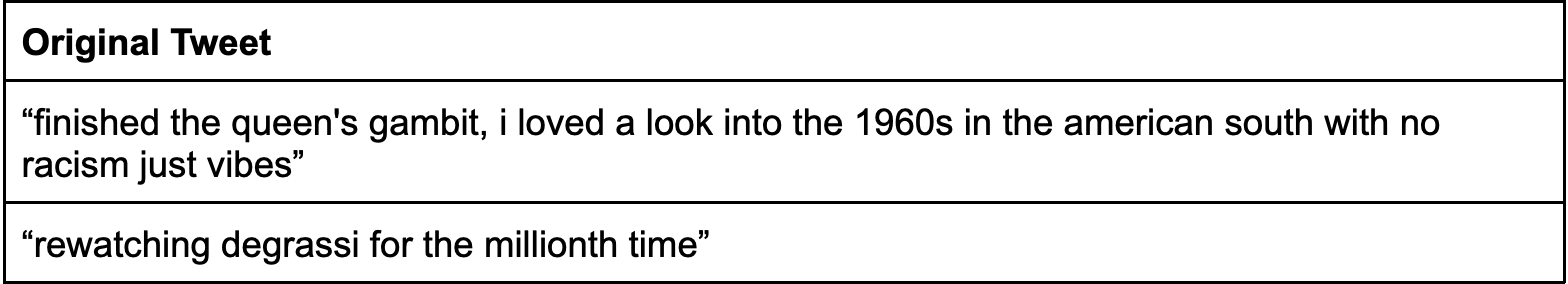
\includegraphics[width=.5\textwidth]{Picture10.png}
    \caption{False negative predictions that required additional contextual information}
    \label{table:false-neg}
\end{figure}


Also, some of the false positives appeared to be mislabeled. In \ref{table:tweets-not-labeled}, we highlight two such examples. In both, we believe that the intended meaning fits the definition of sarcasm, although the tweet is not labeled as such.

\begin{figure}[h!]
    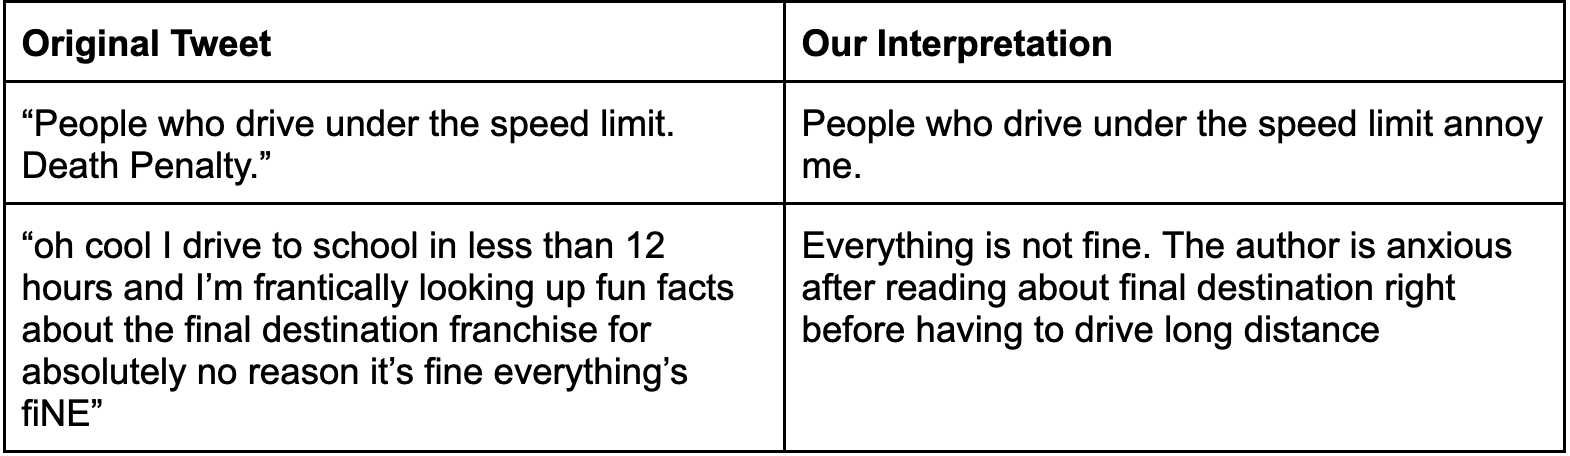
\includegraphics[width=.5\textwidth]{Picture11.png}
    \caption{Tweets not labeled as sarcastic in original dataset that we believe to be sarcastic}
    \label{table:tweets-not-labeled}
\end{figure}

Additionally, there are some false positive examples that lead us to believe the model is learning spurious patterns. In \ref{table:tweets-false-positive}, we highlight two tweets in which neither appear to have sarcastic intent, but were predicted to be sarcastic by our model.

\begin{figure}[h!]
    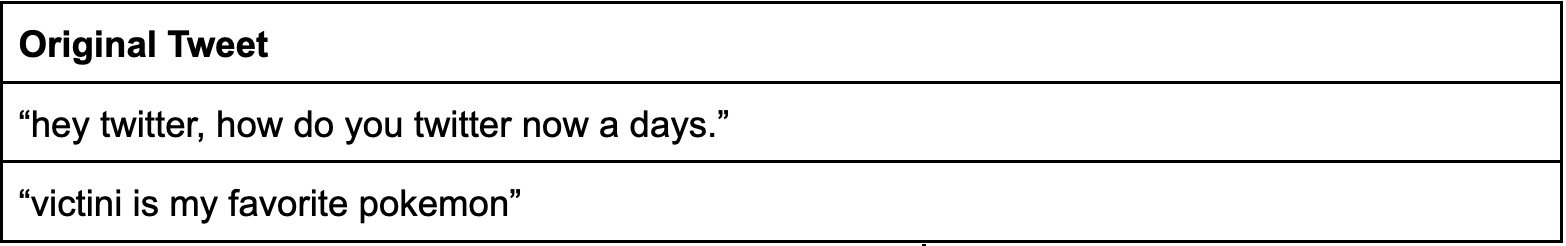
\includegraphics[width=.5\textwidth]{Picture12.png}
    \caption{False positive examples with no clear sarcastic intent}
    \label{table:tweets-false-positive}
\end{figure}


\begin{figure}[h!]
    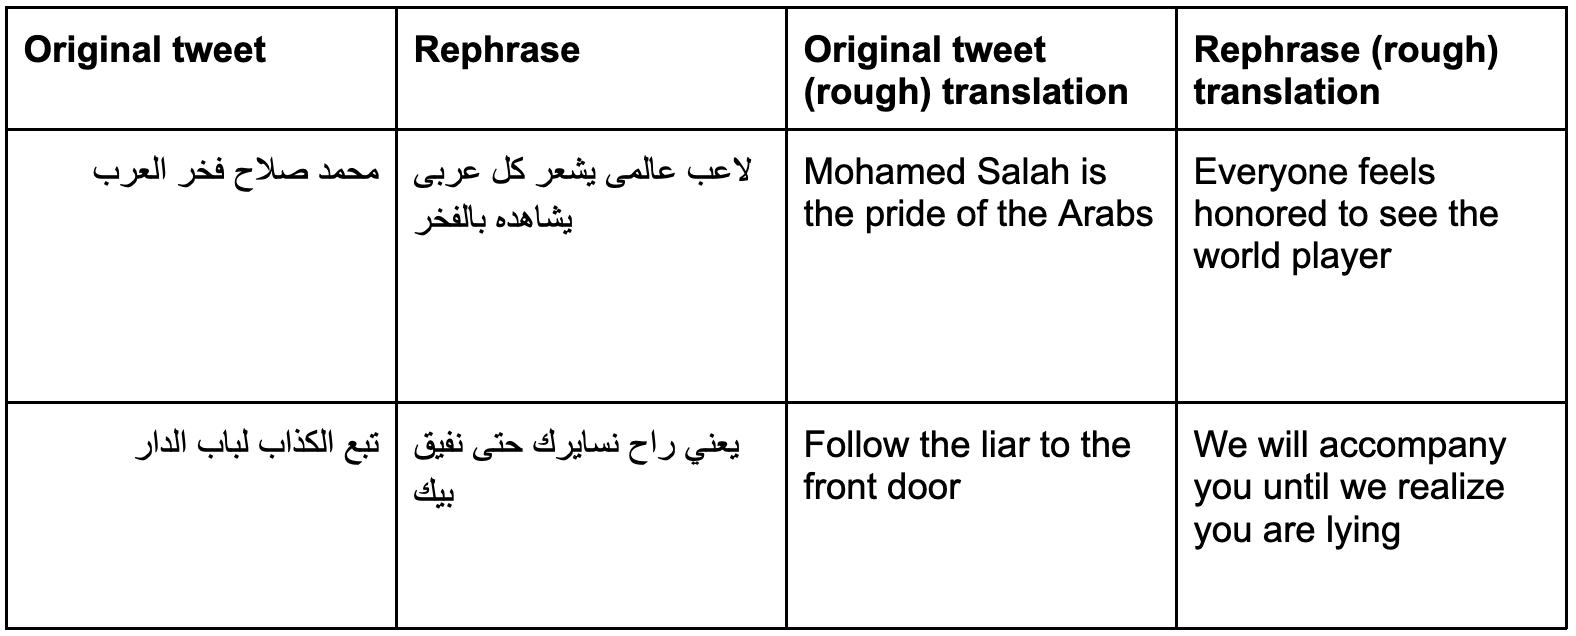
\includegraphics[width=.5\textwidth]{Picture13.png}
    \caption{Tweets labeled as sarcastic believed to not be sarcastic (Arabic dataset)}
    \label{table:tweets-arabic}
\end{figure}


Because none of our team members were Arabic speakers, we faced some challenges when handling the Arabic data. To aid the error analysis of the Arabic data, we consulted a native Arabic speaker from Morocco, who reviewed the data and translated many of the tweets. The reviewer found a large number of tweets that he believed to have been inaccurately labeled as sarcastic, and based on his translations, we agreed. 

The tweets in \ref{table:tweets-arabic} show two examples of tweets from the Arabic that were labeled as sarcastic that our reviewer believed to not be sarcastic. The first tweet in the table roughly translates to "Mohamed Salah is the pride of the Arabs". The rephrasing matches the tweet in both surface-level and underlying meanings, thus not satisfying the criteria for sarcasm. The second tweet in the above table is a well-known proverb, and its rephrasing seems to be the author’s translation of the proverb. These tweets could be considered examples of intended sarcasm that might not be labeled as sarcastic in a perceived sarcasm dataset.

While the reviewer found many tweets that he believed to have been mislabeled as sarcastic, he did not find that any of the non-sarcastic tweets were mislabeled. 



\subsection{Future Work}

With future work on the English portion of the iSarcasmEval task, it may be worthwhile to create a more narrow definition of sarcasm, and remove confusing or mislabeled examples in the iSarcasamEval dataset. Additionally, updating the annotations and labels on the tweets may be helpful as well.

Also, we will attempt to use our system on the Arabic iSarcasmEval dataset. We hope to perform the same sarcasm detection task on the Arabic portion of the dataset, and evaluate our performance by measuring the F1 score on the positive (sarcastic) class.

\section{Conclusion}

In our initial system, the BERTweet model reached an F1 score of .72 on our validation data. 

With our revised system, we used an ensemble of BERTweet-large classifiers, supplemented with data from \citealp{Ptcek2014SarcasmDO}. When evaluating the revised system on our validation data, our ensemble system saw an improvement of .11 F1 over our initial system, with an F1 of .82.

In our adaptation system, we modified our existing system using CamelBERT-mix to detect sarcasm in Arabic. Our adaptation system results were an F1 of .87 on the validation set and .33 on the test set.

\bibliography{anthology,custom}
\bibliographystyle{acl_natbib}

\appendix

\end{document}